\documentclass[12 pt, a4paper]{article}% тип документа, размер шрифта
\usepackage[T2A]{fontenc}%поддержка кириллицы в ЛаТеХ
\usepackage[utf8]{inputenc}%кодировка
\usepackage[russian]{babel}%русский язык
\usepackage{amsmath}%удобная вёрстка многострочных формул, масштабирующийся текст в формулах, формулы в рамках и др.
\usepackage{amsfonts}%поддержка ажурного и готического шрифтов — например, для записи символа {\displaystyle \mathbb {R} } \mathbb {R} 
\usepackage{amssymb}%amsfonts + несколько сотен дополнительных математических символов
\frenchspacing%запрет длинного пробела после точки
\usepackage{setspace}%возможность установки межстрочного интервала
\usepackage{indentfirst}%пакет позволяет делать в первом абзаце после заголовка абзацный отступ
\onehalfspacing%установка полуторного интервала по умолчанию
\usepackage{graphicx}%подключение рисунков
\graphicspath{{figures/}}%путь ко всем рисункам
\usepackage{caption}
\usepackage{float}%плавающие картинки
\usepackage{lastpage}%пакет нумерации страниц
\usepackage{comment}%возможность вставлять большие комменты
\usepackage{multicol}
\usepackage{multirow}
\usepackage{wrapfig} % Пакет для обтекания
\usepackage{booktabs}
\usepackage{siunitx}
\usepackage{array}
\usepackage{xcolor}

%%%%% ПОЛЯ
\setlength\parindent{0pt} 
\usepackage[top = 1.5 cm, bottom = 1.5 cm, left = 1.5 cm, right = 1.5 cm, headheight = 15pt]{geometry}
\setlength\parindent{0pt}

\geometry{top=20mm}
\geometry{bottom=20mm}
\geometry{left=20mm}
\title{}
\author{}
\date{}

\begin{document}
	\begin{titlepage} % начало титульника
		\begin{center}
			\large 13 ноября 2026\\
			\vspace{9.0cm}
			{\LARGE {Лабораторная работа 2\\
					\textbf{Skiplist}}\\}
			\vspace{9.5cm}
			
			\large Сычев Ефим Андреевич, Б02-506\\
			\large 3 семестр
		\end{center}
	\end{titlepage}
	
	% КОНЕЦ ТИТУЛЬНОГО ЛИСТА
	\newpage
	
	\section{Реализация списка с пропусками}

В ходе выполнения работы был написан шаблонный класс \texttt{SkipList<T, Compare>}, реализующий список с пропусками с возможностью задания своего компаратора (по умолчанию используется \texttt{std::less<T>}). Каждый элемент списка представлен структурой \texttt{Node}, в которой хранится само значение \texttt{value}, указатель \texttt{prev} на предыдущий узел нижнего уровня и вектор \texttt{std::vector<Node*> next} с указателями на следующие элементы на каждом из уровней. В начале и в конце списка создаются фиктивные узлы \texttt{head} и \texttt{tail}, за счет которых не нужно отдельно проверять выход за границы при обходе и можно сдвигать итератор \texttt{end()} назад.

Случайная высота нового узла при вставке выбирается с помощью генератора \texttt{std::mt19937} и равномерного распределения \texttt{std::uniform\_real\_distribution<double>(0.0, 1.0)}. Новый элемент всегда добавляется на нижний уровень и с вероятностью $p$ поднимается на уровень выше, пока случайная величина не выпадет больше $p$ или высота не достигнет $K + 1$, где $K$ --- текущее число уровней \texttt{max\_level}.

В классе реализованы конструктор по умолчанию, конструктор с передачей компаратора и вероятности $p$, а также шаблонный конструктор от пары итераторов \texttt{[first, last)}, который позволяет заполнить список из другого контейнера (например, \texttt{std::unordered\_set}). Копирующий конструктор и оператор присваивания поэлементно копируют значения во вновь созданный список, а перемещающий конструктор и перемещающее присваивание работают за $O(1)$, обменивая указатели \texttt{head}, \texttt{tail} и поля класса через метод \texttt{swap()}. Количество элементов хранится в переменной \texttt{elem\_count}, поэтому методы \texttt{size()} и \texttt{empty()} также выполняются за $O(1)$.

Для обхода элементов в отсортированном порядке написан вложенный класс \texttt{iterator} с категорией \texttt{std::bidirectional\_iterator\_tag}, который двигается по нижнему уровню через ссылки \texttt{next[0]} и \texttt{prev}. Обратный итератор \texttt{reverse\_iterator} получен через стандартный адаптер \texttt{std::reverse\_iterator<iterator>}.

Поиск позиции ключа выполняется методами \texttt{lower\_bound} и \texttt{upper\_bound}, которые спускаются с верхнего уровня вниз за $O(\log N)$ и возвращают итератор на первый элемент, не меньший или строго больший заданного ключа. Через них выражены методы \texttt{find}, \texttt{equal\_range} и \texttt{count}. При вставке (\texttt{insert}) одинаковые элементы ставятся после уже добавленных, поэтому \texttt{find} всегда находит первый из дубликатов. Метод удаления \texttt{erase} (по одному итератору и по диапазону) ищет удаляемый узел по совпадению указателя \texttt{Node*} и перекидывает ссылки соседних узлов мимо него, благодаря чему остальные дубликаты и старые итераторы на другие элементы не ломаются.

	\section{Тесты и замеры времени}

Для проверки времени работы вставки, поиска и удаления использовался таймер

\texttt{std::chrono::steady\_clock} (программа компилировалась с флагом оптимизации \texttt{-O2}). Перед каждым запуском массив из $N$ чисел от $0$ до $N-1$ перемешивался в случайном порядке, после чего по очереди замерялось среднее время одной операции \texttt{insert}, \texttt{find} и \texttt{erase} (удаление проводилось по заранее сохраненным итераторам, чтобы не учитывать время повторного поиска). Графики полученных зависимостей показаны на рис.~\ref{fig:bench_n} и~\ref{fig:bench_p}:
\begin{itemize}
    \item \textbf{Зависимость от числа элементов $N$ ($p = 0.5$):} при увеличении размера списка в точках среднее время операций растет: для вставки от $\approx 250$~нс ($N = 1000$) до $\approx 1200$~нс ($N = 500000$), для поиска от $\approx 100$~нс до $\approx 1200$~нс, а для удаления от $\approx 150$~нс до $\approx 1000$~нс.
    \item \textbf{Зависимость от вероятности $p$ ($N = 100\,000$):} наблюдается U-образная зависимость. При малых значениях ($p = 0.05$) время поиска достигает $\approx 2200$~нс (вставка $\approx 1450$~нс, удаление $\approx 1800$~нс). В диапазоне оптимума $p \in [0.3, 0.7]$ время стабилизируется и составляет $\approx 400$--$600$~нс для всех операций. При росте до $p = 0.95$ время вставки увеличивается до $\approx 1100$~нс (поиск $\approx 1000$~нс, удаление $\approx 900$~нс) из-за избыточной высоты узлов.
\end{itemize}

\begin{figure}[H]
    \centering
    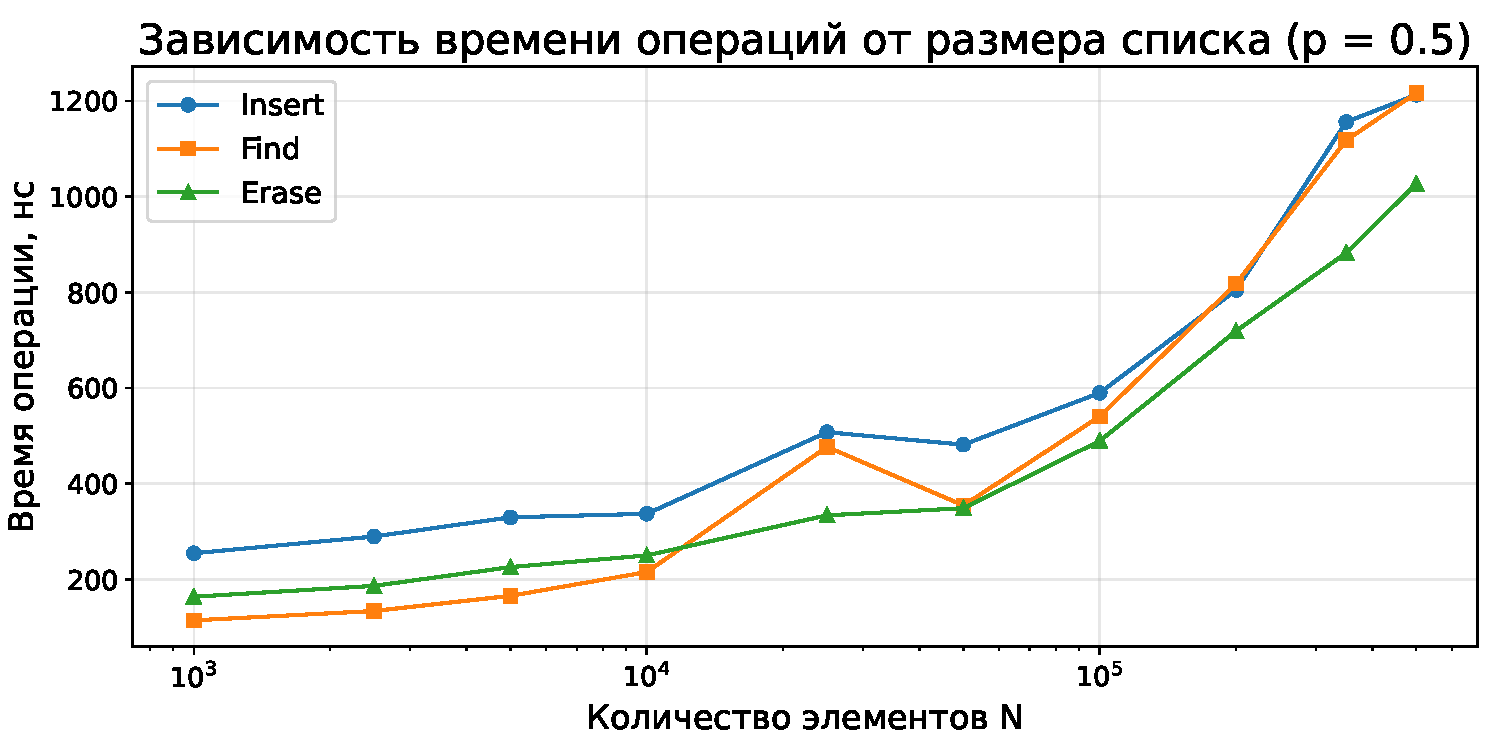
\includegraphics[width=\textwidth]{bench_n.pdf}
    \caption{Зависимость среднего времени операций \texttt{insert}, \texttt{find} и \texttt{erase} от количества элементов $N$ при $p = 0.5$}
    \label{fig:bench_n}
\end{figure}

\begin{figure}[H]
    \centering
    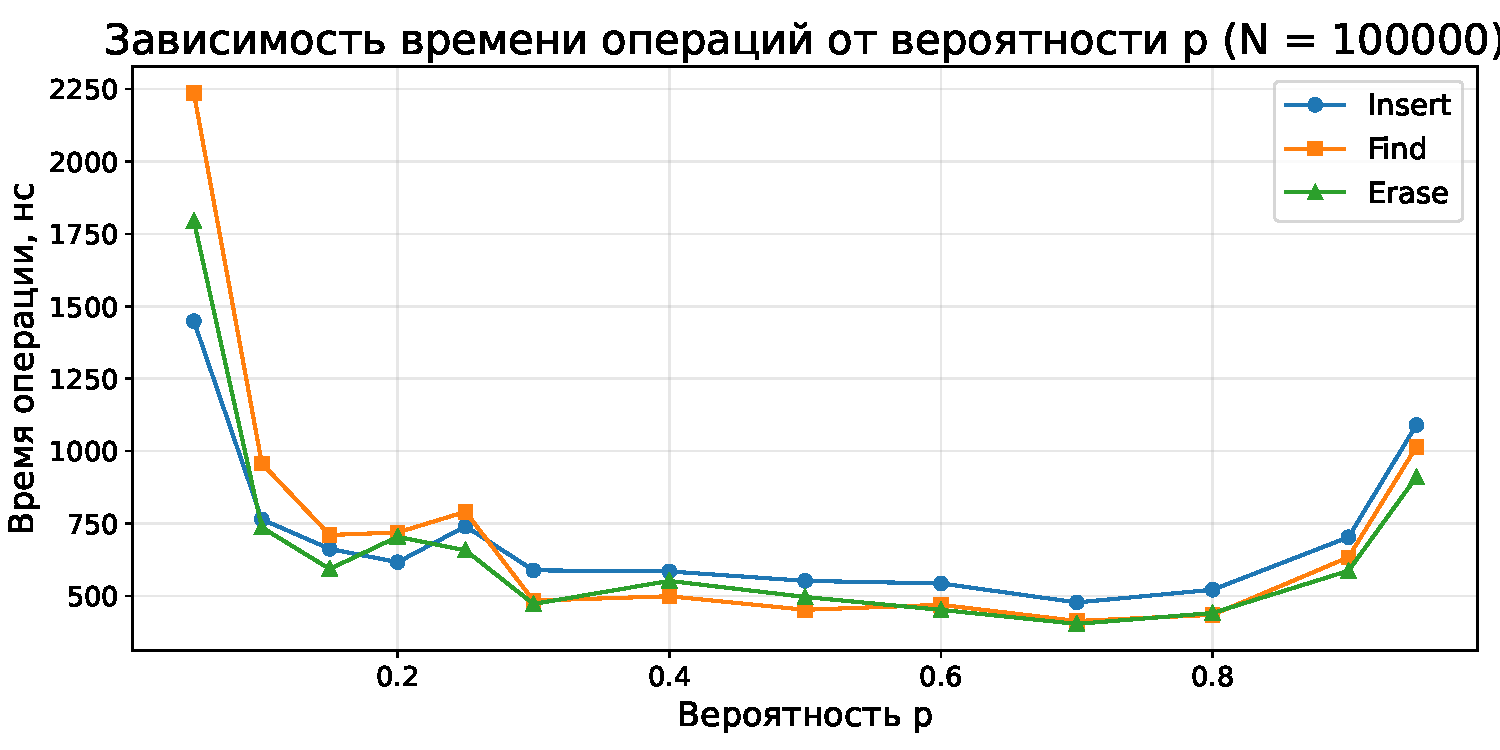
\includegraphics[width=\textwidth]{bench_p.pdf}
    \caption{Зависимость среднего времени операций \texttt{insert}, \texttt{find} и \texttt{erase} от вероятности $p$ при $N = 100\,000$}
    \label{fig:bench_p}
\end{figure}

\end{document}